\section{Jet flavour tagging}
\label{sec:ch6_btag}

Jet flavour tagging is used to distinguish $b$-quark originating jets ($b$-jets) from other jet flavours.

$b$-jets are identified through displaced $b$-hadron decays, which have a lifetime of about $1.5$~ps. Therefore a boosted $b$-hadron can travel several millimetres before decaying~\cite{ATLAS2026GN2}.
The decay tracks therefore tipically have large impact parameters and originate from a secondary vertex displaced from the PV.
Charm hadrons produced in the $b$-hadron decay can further decay at an additional displaced vertex.
These features are used for jet flavour tagging.

The tagger uses the GN2v01 algorithm, which is based on a transformer neural network~\cite{ATLAS2026GN2}.
Its inputs include jet kinematics, track impact parameters and hit variables.
Within the transformer, information from other tracks in the jet is used to update the representation of each track.
Correlations between tracks can thereby be used to recognise a common displaced origin without requiring explicitly reconstructed secondary vertices as separate inputs.
During training, the jet-flavour classification is supplemented by two auxiliary tasks: identifying track origins and determining which tracks originate from the same vertex.
The shared network and its three tasks are illustrated in Figure~\ref{fig:ch6_gn2}.

Four classifier outputs are obtained for the $b$-jet, $c$-jet, hadronic-$\tau$ and light-jet hypotheses, where light jets originate from $u$, $d$ or $s$ quarks or gluons.
These outputs are combined into a single discriminant, $D_b$, which compares the $b$-jet output with a weighted combination of the other three outputs.
Larger values favour the $b$-jet hypothesis~\cite{ATLAS2026GN2}.
The GN2v01 85\% working point is used in this analysis.
A jet is tagged when $D_b$ exceeds a fixed threshold corresponding to a nominal $b$-jet tagging efficiency of 85\%.
The efficiency depends on the jet kinematics and can therefore differ in the signal samples.

\begin{figure}[htbp]
    \centering
    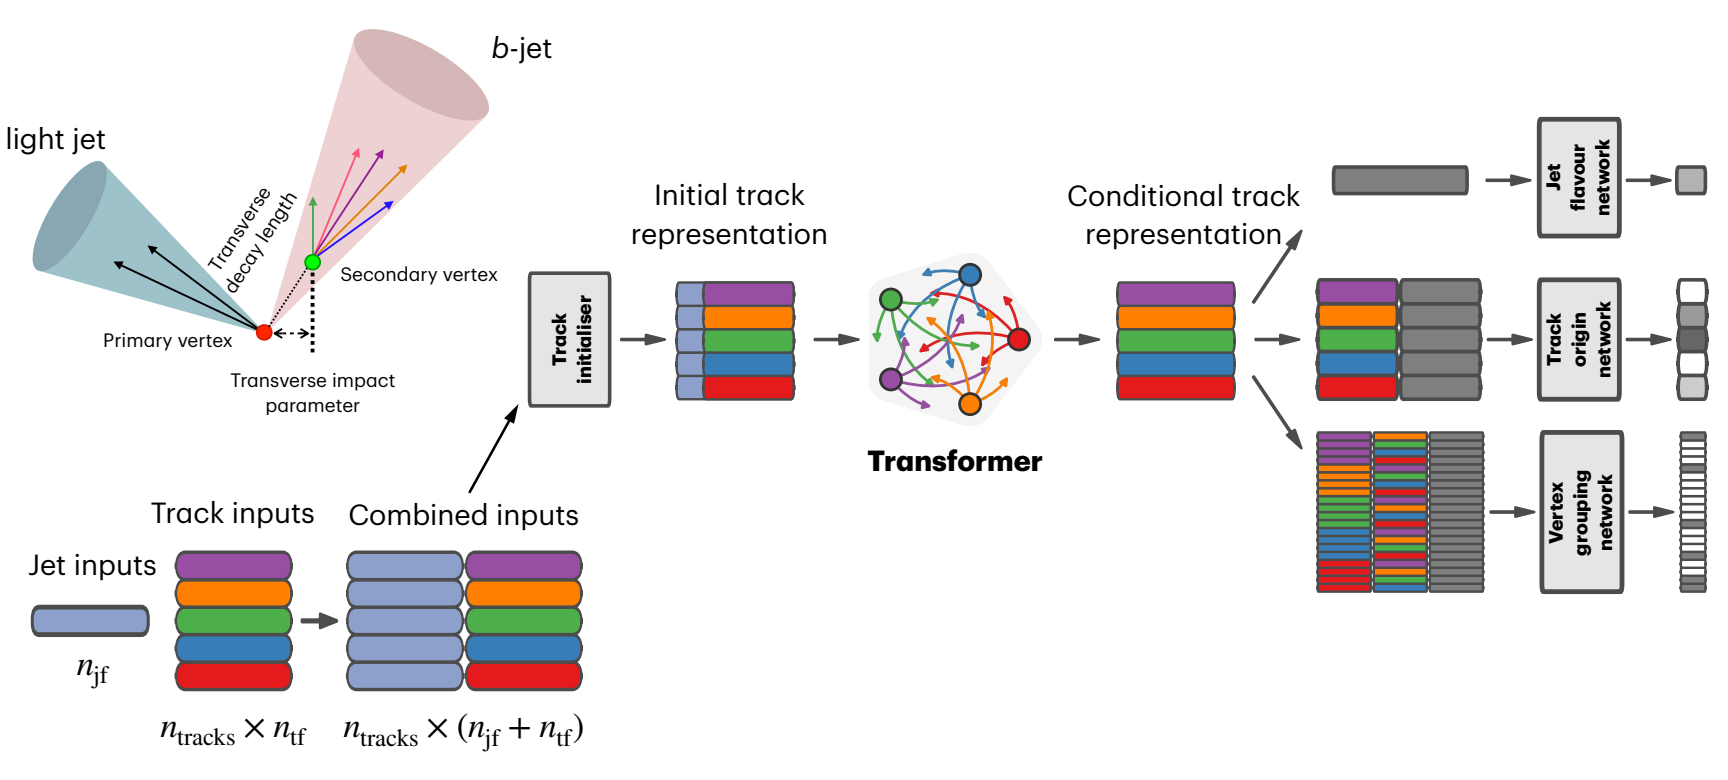
\includegraphics[width=\textwidth]{output/ch6/figures/gn2_architecture.png}
    \caption[GN2 flavour-tagging architecture]{GN2 flavour-tagging architecture. Jet and track measurements are combined, processed by the transformer, and used for jet-flavour prediction and the auxiliary track-origin and vertex-grouping tasks. The symbols $n_{\mathrm{jf}}$, $n_{\mathrm{tf}}$ and $n_{\mathrm{tracks}}$ denote the numbers of jet features, track features and tracks~\cite{ATLAS2026GN2}.}
    \label{fig:ch6_gn2}
\end{figure}

\subsection{Calibration}

The $b$-jet tagging efficiency and the $c$-jet and light-jet mistagging efficiencies are measured in flavour-enriched data samples and compared with simulation~\cite{ATLAS2026GN2}.
The corresponding scale factors are defined as in Eq.~\ref{eq:ch6_efficiency_sf} and depend on the jet flavour and kinematics.
A tagged jet of flavour $f$ is assigned a weight $\mathrm{SF}_f$.
Untagged jets also require a correction because the probability for a jet to fail the tag is $1-\epsilon_f$, where $\epsilon_f$ is the tagging efficiency for flavour $f$.
The weight for an untagged jet is therefore
\begin{align}
    w_f^{\mathrm{untagged}}
    =\frac{1-\epsilon_f^{\mathrm{data}}}{1-\epsilon_f^{\mathrm{MC}}}
    =\frac{1-\mathrm{SF}_f\epsilon_f^{\mathrm{MC}}}{1-\epsilon_f^{\mathrm{MC}}},
    \label{eq:ch6_btag_untagged}
\end{align}
where $\epsilon_f^{\mathrm{data}}$ and $\epsilon_f^{\mathrm{MC}}$ are the efficiencies in data and simulation, respectively.
The simulated event weight is multiplied by the product of the factors for its tagged and untagged jets.
Flavour-tagging corrections therefore affect both the zero-tag and tagged event categories.
